
\begin{figure}
    \centering
    \begin{subfigure}[b]{0.45\textwidth}
        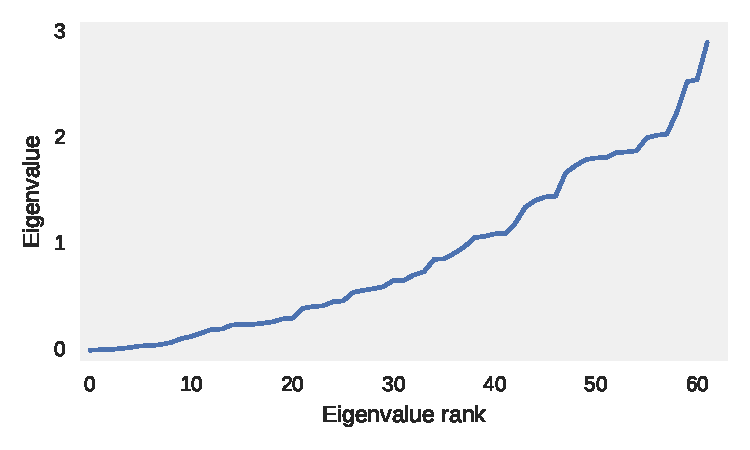
\includegraphics[width=\textwidth]{FishPoo/figures/gopher_louse_eigenvalues}
        \small
        \caption{Eigenvalues of graph Laplacian}
    \end{subfigure}
    \begin{subfigure}[b]{0.45\textwidth}
        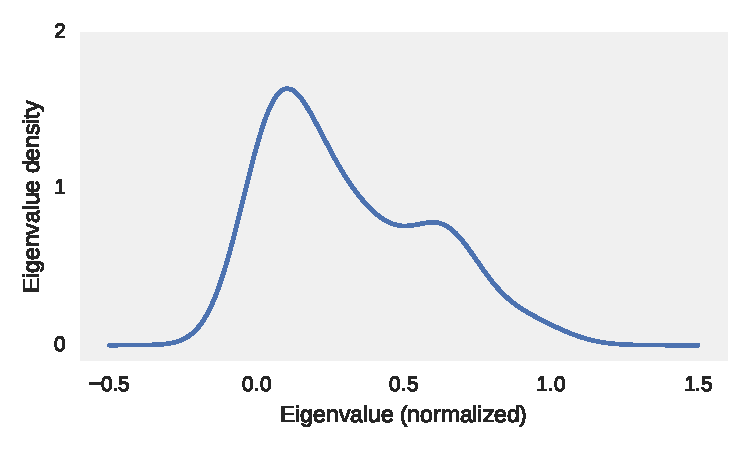
\includegraphics[width=\textwidth]{FishPoo/figures/gopher_louse_spectral_density}
        \small
        \caption{Spectral density of eigenvalues}
    \end{subfigure}
    \caption{Eigenvalues in rank order of the graph Laplacian matrix of interactions among pocket gophers and their chewing lice parasites from Hafner {\em et al.} \cite{hafner1994disparate} \textbf{(a)} and the normalized density distribution of eigenvalues computed with a kernel density estimator using a Gaussian bandwidth of 0.4 \textbf{(b)}. }
    \label{fig:FP_eigendensity}
\end{figure}